\chapter{Solving Strategies}
\label{chap:strategies}

This chapter describes and compares different strategies and approaches used and tested during solver development.


%%%%%%%%%%%%%%%%%%%%%%%%%%%%%%%%%%%%%%%%%%%%%%%%%%%%%%%%%%%%%%%%%%%%%%%%%%%%%%%%%%
\section{Goal programming}

Just as in any other kind of problem, the feasibility of a linear model for a timetabling problem depends utterly on data set. In general, there is no guarantee that all demanded requirements can be satisfied with the specified available resources, even because usually there are several and conflicting objectives. Therefore, specially in a commercial solver, it is important to treat some idealistic hard constraints as highest priority soft constraints, otherwise the solver could frequently generate an infeasible model.

In real life it is useless for an educational institution to have a solution that satisfies all demands of students for courses, but which does not respect some important quality requirements. Bearing this in mind, in addition to the feasibility issue, the model presented at this work, unlike most authors, does not consider demand satisfaction as a hard constraint. Essential quality requirements are modeled as hard constraints though, and demand satisfaction is treated as the highest priority objective, followed by some further goals.

While it is not easy to embody quality into the modeling process, it can be even more difficult to quantify it. A \textbf{multi-objective function} unifies disparate goals of the model in a single weighted sum of preferences. Such approach, although simpler, depends on very subjective choice of weights and is not always consistently reliable, specially when objectives are mutually conflicting.

An alternative approach is using a priority line for the different goals. According to the institution preferences, one optimizes the problem in a sequence of steps, where each step is responsible for a goal, from the most to the least important. For each step a different and specific objective function is used and the feasible solution space is subject to features of the best solution found at the previous step. Such approach is known as \textbf{preemptive goal programming} and is following detailed.


%%%%%%%%%%%%%%%%%%%%%%%%%%%%%%%%%%%%%
\subsection{General concept}

A goal programming model seeks to simultaneously take into account several objectives or goals that are concern to a decision maker. While a linear programming model consists of constraints and a single objective function to be maximized or minimized, a goal programming model consists of constraints and a set of goals that are prioritized in some sense.
In both linear and goal programming problems, if the constraints are inconsistent, there are no feasible solutions for the model. In goal programming, however, one can expect that although there is a set of feasible solutions satisfying the constraints, none of them may simultaneously satisfy all the conflicting goals of the organization. The objective of goal programming is to find a solution that satisfies the true constraints and comes closest to meeting the stated goals.

In \textbf{lexicographic} or \textbf{preemptive goal programming} the decision maker orders the unwanted deviations into a number of priority levels, with the minimization of a deviation in a higher priority level being infinitely more important than any deviations in lower priority levels. A lexicographic goal program can be solved as a series of linear programs and should be used when there is a clear priority ordering amongst the goals to be achieved. The idea behind the preemptive goal programming approach is that lower priority level goals should not be attained at the expense of higher priority goals --- they are preempted.

If the decision maker is more interested in direct comparisons of the objectives then weighted or \textbf{nonpreemptive goal programming} should be used. In this case all the unwanted deviations are multiplied by weights, reflecting their relative importance, and added together as a single sum to form the achievement function, which converts the goal programming model into a linear programming model.

G\"{u}enalay and Sahin use goal programming at \cite{Guenalay2006} to satisfy instructors' preferences as much as possible.


%%%%%%%%%%%%%%%%%%%%%%%%%%%%%%%%%%%%%
\subsection{Applying Goal Programming}

%%%%%%%%%%%%%%
\subsubsection{Preemptive Goal Programming}

Following are listed the goals, ordered by priority, considered at this work when using preemptive goal programming. For each step there is a specific objective function and the respective feasible solution space is additionally constrained by the solution of the previous phase. We draw attention to the ease of changing priorities order and adding or removing goals; and to the nonexistence of coefficients multiplying variables at each objective function.

\begin{enumerate}

%%%%%
\item{Maximizing demand satisfaction}

\begin{align*}
   \mbox{g1 = MIN  } \sum\limits_{a \in A}\sum\limits_{d \in D} fd_{d,a}
\end{align*}

%%%%%
\item{Minimizing virtual professor usage}

\begin{align*}
  \mbox{g2 = MIN  } \sum\limits_{i \in I_{d}} \sum\limits_{d \in D} \sum\limits_{cp \in CP} y_{pv,i,d,cp}
	\\
	\sum\limits_{a \in A}\sum\limits_{d \in D} fd_{d,a} \le g1
\end{align*}

Where the additional constraint restricts the solution space to the maximum demand achieved at previous step.

%%%%%
\item{Minimizing real professor displacement}

\begin{align*}
  \mbox{g3 = MIN  } \sum\limits_{p \in P} \sum\limits_{t \in T} \sum\limits_{u1 \in U} \sum\limits_{u2 \in U} Time_{u1,u2} \cdot desloc_{p,t,u1,u2}
	\\
	\sum\limits_{a \in A}\sum\limits_{d \in D} fd_{d,a} \le g1
	\\
	\sum\limits_{i \in I_{d}} \sum\limits_{d \in D} \sum\limits_{cp \in CP} y_{pv,i,d,cp} \le g2
\end{align*}

Where the additional constraint restricts the solution space to the minimum virtual professor usage achieved at previous step.

%%%%%
\item{Minimizing gaps in professor's timetable}

\begin{align*}
   \mbox{g4 = MIN  } \sum\limits_{p \in P} \sum\limits_{t \in T} \sum\limits_{f \in F} fpgap_{p,t,f}
	\\
	\sum\limits_{a \in A}\sum\limits_{d \in D} fd_{d,a} \le g1
	\\
	\sum\limits_{i \in I_{d}} \sum\limits_{d \in D} \sum\limits_{cp \in CP} y_{pv,i,d,cp} \le g2
	\\
	\sum\limits_{p \in P} \sum\limits_{t \in T} \sum\limits_{u1 \in U} \sum\limits_{u2 \in U} Time_{u1,u2} \cdot desloc_{p,t,u1,u2} \le g3
\end{align*}

Where the additional constraint restricts the solution space to the minimum real professor displacement achieved at previous step.

%%%%%
\item{Minimizing usage of further slack variables}

\begin{align*}
   \mbox{g5 = MIN  } \sum\limits_{d \in D} \sum\limits_{t \in T} \sum\limits_{i \in I_{d}} (fkp_{d,i,k} + fkm_{d,i,k})
	\\
	\sum\limits_{a \in A}\sum\limits_{d \in D} fd_{d,a} \le g1
	\\
	\sum\limits_{i \in I_{d}} \sum\limits_{d \in D} \sum\limits_{cp \in CP} y_{pv,i,d,cp} \le g2
	\\
	\sum\limits_{p \in P} \sum\limits_{t \in T} \sum\limits_{u1 \in U} \sum\limits_{u2 \in U} Time_{u1,u2} \cdot desloc_{p,t,u1,u2} \le g3
	\\
	\sum\limits_{p \in P} \sum\limits_{t \in T} \sum\limits_{f \in F} fpgap_{p,t,f} \le g4
\end{align*}


Where the additional constraint restricts the solution space to the minimum amount of gaps in professors' timetable achieved at previous step.

\end{enumerate}

The final solution is the one with cost equal to $g5$, achieved at last stage. If an optimal solution is achieved for all steps, then at the end of the last step we guarantee that the final solution found is the best one with respect to the order of priorities.


\begin{figure}[h]
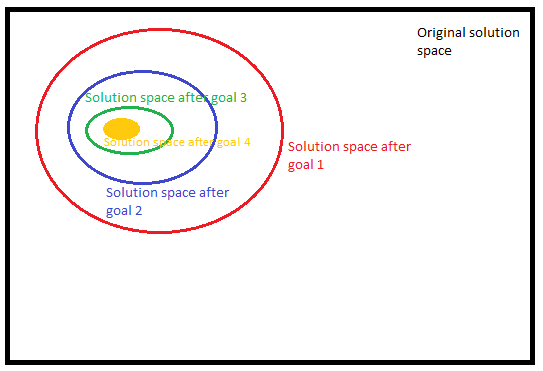
\includegraphics[scale=0.6]{figures/goalProgSpace.png}
\centering
\caption{Solution spaces are limited and encapsulated after each goal optimization step.}
\end{figure}

\fixme{atualizar etapas na figura}


%%%%%%%%%%%%%%
\subsubsection{Nonpreemptive Goal Programming}
\fixme{or Multi-objective function? no final nao tem mta diferenca!}

Following there is the unified objective function considered at this work. Although here it is even easier than at goal programming to change priorities order and adding or removing goals, there is the necessity of choosing coefficients for variables at objective function.

$$
\begin{array}{rl}
   \mbox{MIN} &
			\lambda \cdot \sum\limits_{a \in A}\sum\limits_{d \in D} \cdot fd_{d,a}
      \\
      &
      + \omega \cdot \sum\limits_{d \in D} 
\sum\limits_{t \in T} \sum\limits_{i \in I_{d}} (fkp_{d,i,k} + fkm_{d,i,k})
      \\
      &
      + \epsilon \cdot \sum\limits_{p \in P} \sum\limits_{t \in T} \sum\limits_{f \in F} fpgap_{p,t,f}
      \\
      &
			+ \sigma \cdot \sum\limits_{p \in P} \sum\limits_{t \in T} \sum\limits_{u1 \in U} \sum\limits_{u2 \in U} Time_{u1,u2} \cdot desloc_{p,t,u1,u2}
			\\
			&
      + \theta \cdot \sum\limits_{i \in I_{d}} \sum\limits_{d \in D} \sum\limits_{cp \in CP} y_{pv,i,d,cp}
\end{array}
$$


An unified objective function is more appropriate when goals have not a strict priority order, in the sense that their combinations can produce solutions that are Pareto efficient.

So, the question when choosing the approach is whether one wants to order or weight goals.


%%%%%%%%%%%%%%%%%%%%%%%%%%%%%%%%%%%%%
\subsection{Comparing results}

Through preemptive goal programming it is easier to understand the best solution found by the optimization process and the reasons of non-satisfaction of different goals, specially when the number of goals to be achieved through the objective function increases.





%%%%%%%%%%%%%%%%%%%%%%%%%%%%%%%%%%%%%%%%%%%%%%%%%%%%%%%%%%%%%%%%%%%%%%%%%%%%%%%%%%%%%%%%%%%%%%%%%%%
%%%%%%%%%%%%%%%%%%%%%%%%%%%%%%%%%%%%%%%%%%%%%%%%%%%%%%%%%%%%%%%%%%%%%%%%%%%%%%%%%%%%%%%%%%%%%%%%%%%
\section{Polishing Method}

%%%%%%%%%%%%%%%%%%%%%%%%%%%%%%%
\subsection{Definition}

Introduces polishing concept.

%%%%%%%%%%%%%%%%%%%%%%%%%%%%%%%%%%%%%
\subsection{Polishing method developed for the problem}

\begin{algorithm}
  \caption{Polishing method
    \label{alg:polishing}}
  \begin{algorithmic}[1]
    \Require{$lp$ model and any initial feasible solution $xSol$}
    \Statex
    \Function{Polish}{$xSol$, $percIni$, $maxTime$, $maxTimeNoImprov$}
		
			\State $init()$
      \Let{$perc$}{$percIni$}
      \State $setParams(timeIter)$
			\Let{$okIter$}{$true$}
      \While{$okIter$}
          \State $fixVars()$
					\State $optimize()$
					\State $double objN, gap$
					\State $getSolution(objN, gap)$
					\State $setMelhora(objN)$
					\State $updatePercAndTimeIter(objN, gap)$
					\State $checkTimeWithoutImprov(objN)$
					\State $updateObj(objN)$
					\State $checkTimeLimit()$
					\State $unfixVars()$
      \EndWhile
     \State \Return{$xSol$}
    \EndFunction
  \end{algorithmic}
\end{algorithm}
		  	  

\begin{algorithm}
  \caption{Fixing Variables' Values
    \label{alg:fixVars}}
  \begin{algorithmic}[1]
    \Require{$lp$ model and a feasible solution $xSol$}
    \Procedure{fixVars}{$xSol$, $perc$}
			\State $fixUnidsTatico()$
			\State $clearVarsToFixType1()$
			\State $decideVarsToFixByPhase()$
			\State $fixVarsType1()$
			\State $fixVarsProfType1()$
      \State \Return{$xSol$}
    \EndProcedure
	\Statex	
  \Algphase{Fixing Blocks}
    \Require{$lp$ model and a feasible solution $xSol$}
    \Procedure{fixUnidsTatico}{$lp$, $xSol$, $percUnid$}
			 \State
			 \Forall{variable $x \in lp$ such that the associated block is fixed}
				\Let{$LB_{x}$}{$xSol[x]$}
				\Let{$UB_{x}$}{$xSol[x]$} 
			 \EndFor
    \EndProcedure
	\Statex
  \Algphase{Decide which variable to fix}
    \Require{$lp$ model, a feasible solution $xSol$ and a percentage $perc$ of classes to be fixed}
    \Function{decideVarsToFixByPhase}{$lp$, $xSol$, $perc$}
			\Let{$F$}{$\emptyset$}
			\Forall{variable $z \in lp$}
					\If{rand() \ge perc}
						\Let{$F$}{$z$}
					\EndIf
			\EndFor
			\Return F
    \EndFunction
	\Statex
	\Algphase{Fix variables of lessons}
    \Require{$lp$ model, a feasible solution $xSol$ and a set $F$ of classes to be fixed}
    \Procedure{fixVarsType1}{$lp$, $xSol$, $F$}
			\State
			 \Forall{variable $x \in F$}
				\Let{$LB_{x}$}{$xSol[x]$}
				\Let{$UB_{x}$}{$xSol[x]$} 
			 \EndFor
    \EndProcedure	
	\Statex
	\Algphase{Fix variables of professors}
    \Require{$lp$ model and a feasible solution $xSol$}
    \Procedure{fixVarsProfType1}{$lp$, $xSol$, $perc$}
			\Forall{variable $y \in lp$}
					\If{rand() \ge perc}
						\Let{$LB_{y}$}{$xSol[y]$}
						\Let{$UB_{y}$}{$xSol[y]$} 
					\EndIf
			\EndFor
    \EndProcedure	
  \end{algorithmic}	
\end{algorithm}



\begin{algorithm}
  \caption{Set free and fixed blocks for the next iteration
    \label{alg:setNextRandFreeUnidade}}
  \begin{algorithmic}[1]
    \Require{$lp$ model}
    \Statex
    \Procedure{setNextRandFreeUnidade}{$adjustPercUnid$}
			\State adjustPercFreeUnid$(adjustPercUnid)$
      \If{there is enough consecutive iterations with fixed blocks}
      	\State free all blocks for the next iteration
      	\Return
      \End
      \State chooseAndSetFreeUnidades()
    \EndProcedure
	\Statex
	\Algphase{Fix variables of professors}
    \Require{$lp$ model}
    \Procedure{chooseAndSetFreeUnidades}{}
			\State clearFreeUnidade()
			\State decideTypeOfUnidToFree()
			\If {type of fixing blocks is per cluster}
				\State chooseClusterAndSetFreeUnidade()
			\EndIf
			\State chooseRandAndSetFreeUnidade()
    \EndProcedure	    
  \end{algorithmic}
\end{algorithm}





%%%%%%%%%%%%%%%%%%%%%%%%%%%%%%%%%%%%%
\subsection{Comparing different approaches}

%%%%%%%%%%%%%%%%%%%%%%%%%%%%%%%%%%%%%
\subsubsection{Fixing types}




%%%%%%%%%%%%%%%%%%%%%%%%%%%%%%%%%%%%%%%%%%%%%%%%%%%%%%%%%%%%%%%%%%%%%%%%%%%%%%%%%%%%%%%%%%%%%%%%%%%
%%%%%%%%%%%%%%%%%%%%%%%%%%%%%%%%%%%%%%%%%%%%%%%%%%%%%%%%%%%%%%%%%%%%%%%%%%%%%%%%%%%%%%%%%%%%%%%%%%%
\section{Root relaxation}

%%%%%%%%%%%%%%%%%%%%%%%%%%%%%%%%%%%%%
\subsection{Barrier method vs primal method algorithms}




%%%%%%%%%%%%%%%%%%%%%%%%%%%%%%%%%%%%%%%%%%%%%%%%%%%%%%%%%%%%%%%%%%%%%%%%%%%%%%%%%%%%%%%%%%%%%%%%%%%
%%%%%%%%%%%%%%%%%%%%%%%%%%%%%%%%%%%%%%%%%%%%%%%%%%%%%%%%%%%%%%%%%%%%%%%%%%%%%%%%%%%%%%%%%%%%%%%%%%%
\section{Different mathematical formulation}

%%%%%%%%%%%%%%%%%%%%%%%%%%%%%%%%%%%%%
\subsection{Single time slot variable vs grouping time slot variable}



As in all combinatorial scheduling models, the problem grows more complex as the number of side constraints increases.\fixme{Colocar essa frase no lugar adequado!}



%%%%%%%%%%%%%%%%%%%%%%%%%%%%%%%%%%%%%%%%%%%%%%%%%%%%%%%%%%%%%%%%%%%%%%%%%%%%%%%%%%%%%%%%%%%%%%%%%%%
%%%%%%%%%%%%%%%%%%%%%%%%%%%%%%%%%%%%%%%%%%%%%%%%%%%%%%%%%%%%%%%%%%%%%%%%%%%%%%%%%%%%%%%%%%%%%%%%%%%
\section{Usage of virtual resource}

%%%%%%%%%%%%%%%%%%%%%%%%%%%%%%%%%%%%%
\subsection{Virtual professor vs no virtual professors}

